\chapter{Complex bends}
\label{complexbends}
Now that we have built up the foundation of how we can force a wave to
propagate in a specific direction in a topologically repeating material or
metamaterial, we want to see just how robust this phenomenon is based on the
shape of the boundary, i.e. just how much can we bend the wave?

\textit{Note:} For the hexagonal simulations, we will specifically be using the
same top and bottom cells as Figure~\ref{fig:hexstdrotstraight}, which is with
alternating masses as defined in Figure~\ref{fig:hexstripMrotated}. And for the
kagome simulations, we will specifically be using the same top and bottom cells
as Figure~\ref{fig:kagomestd}.

\section{Gentle and sharp straight bends}
So far we have seen just straight line boundaries, but can this work for bent
boundaries too? Due to the way we set up our lattice (with the strips getting
higher as we go from left to right), there are two kinds of bends we can make
straight away. The 'gentle' bend where we bend the boundary upwards, and the
'sharp' bend where we bend the boundary downwards.

\begin{figure}[!h]
\centering
\begin{subfigure}[b]{.5\textwidth}
  \centering
  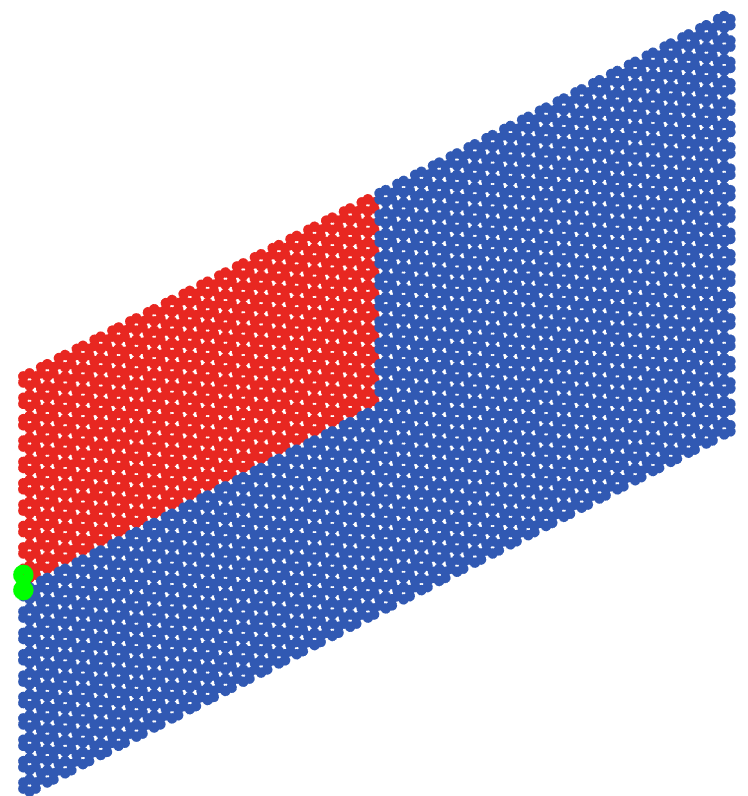
\includegraphics[width=0.8\linewidth]{imgs/gentlebendarr.png}
  \caption{Arrangement of cells to form a gentle bend.}
  \label{fig:sub1}
\end{subfigure}%
\begin{subfigure}[b]{.5\textwidth}
  \centering
  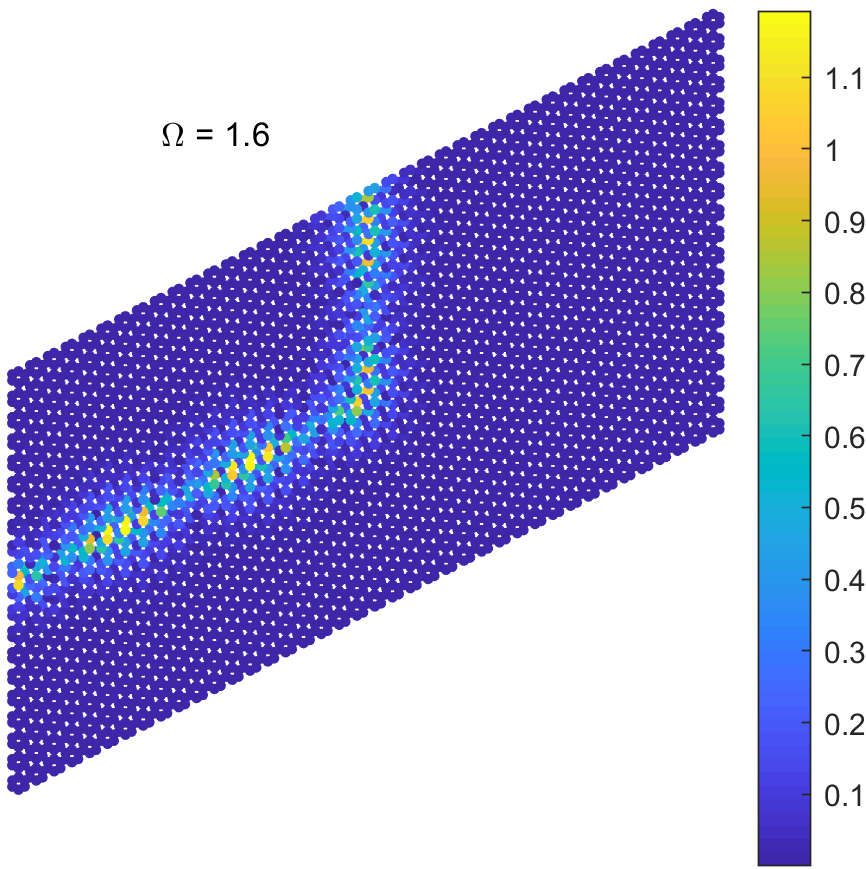
\includegraphics[width=1\linewidth]{imgs/gentlebendscat.png}
  \caption{The plot of $|y_i|$ for each mass in each cell.}
  \label{fig:sub2}
\end{subfigure}

\medskip
\centering
\begin{subfigure}[b]{.5\textwidth}
  \centering
  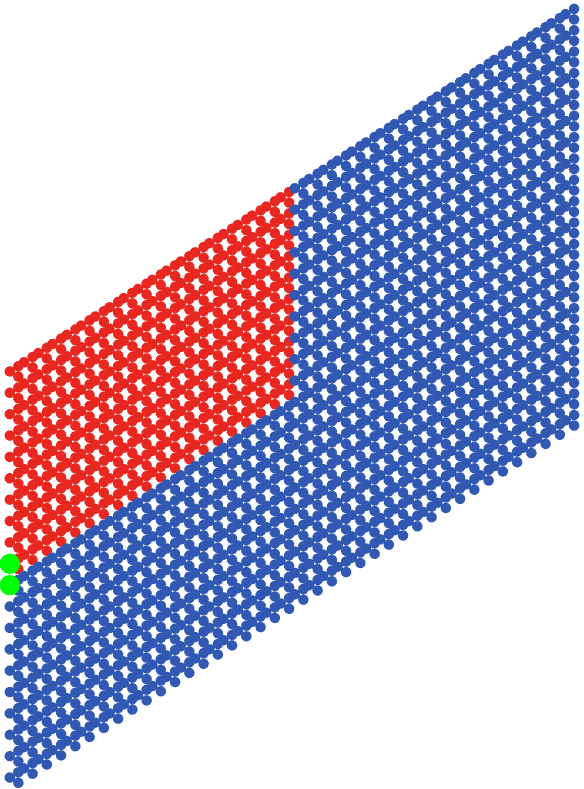
\includegraphics[width=0.8\linewidth]{imgs/kagomegentlebendarr.png}
  \caption{Arrangement of cells to form a gentle bend.}
  \label{fig:sub1}
\end{subfigure}%
\begin{subfigure}[b]{.5\textwidth}
  \centering
  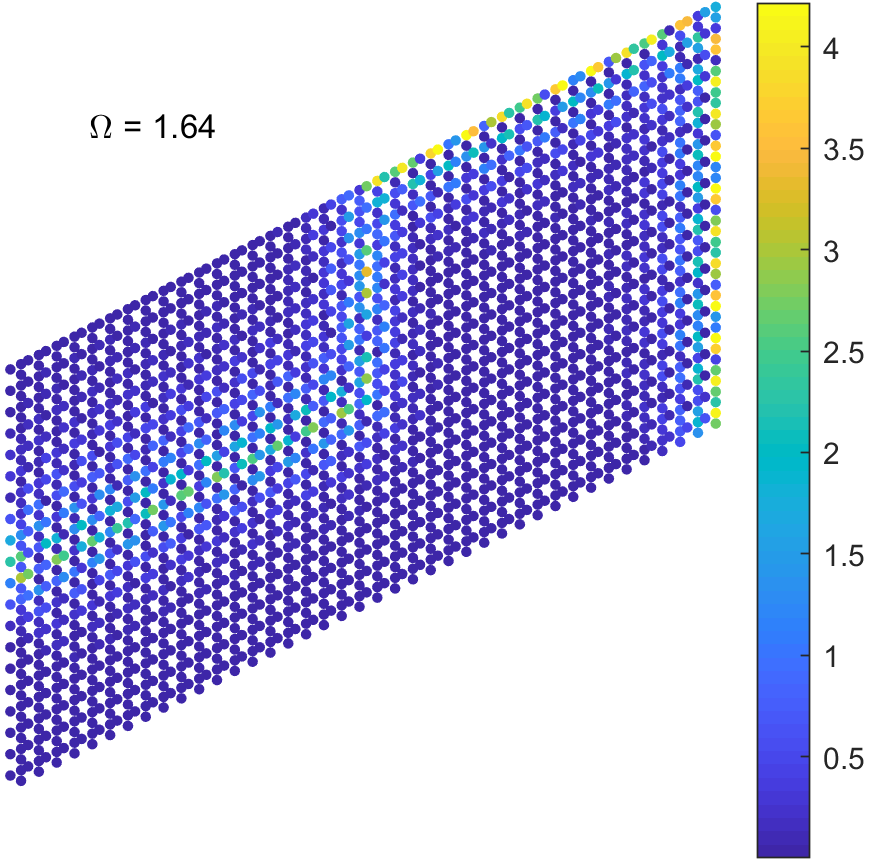
\includegraphics[width=1\linewidth]{imgs/kagomegentlebendscat.png}
  \caption{The plot of $|y_i|$ for each mass in each cell.}
  \label{fig:kagomegentlebendscat}
\end{subfigure}
\caption{Simulation of scattering hexagonal and kagome finite lattices with a
  gentle bend.}
\label{fig:gentlebend}
\end{figure}

\begin{figure}[!h]
\centering
\begin{subfigure}[b]{.5\textwidth}
  \centering
  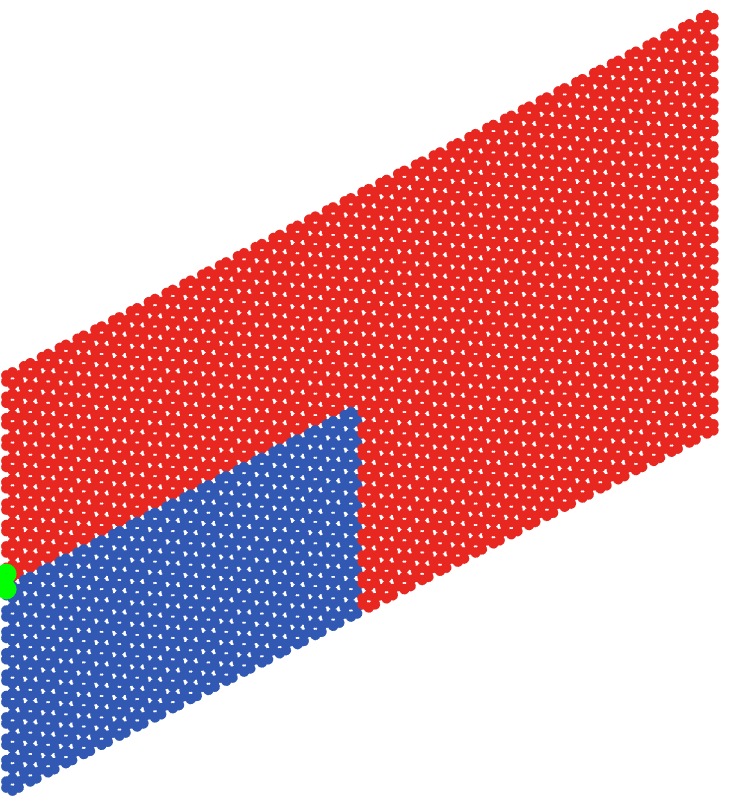
\includegraphics[width=0.8\linewidth]{imgs/sharpbendarr.png}
  \caption{Arrangement of cells to form a sharp bend.}
  \label{fig:sub1}
\end{subfigure}%
\begin{subfigure}[b]{.5\textwidth}
  \centering
  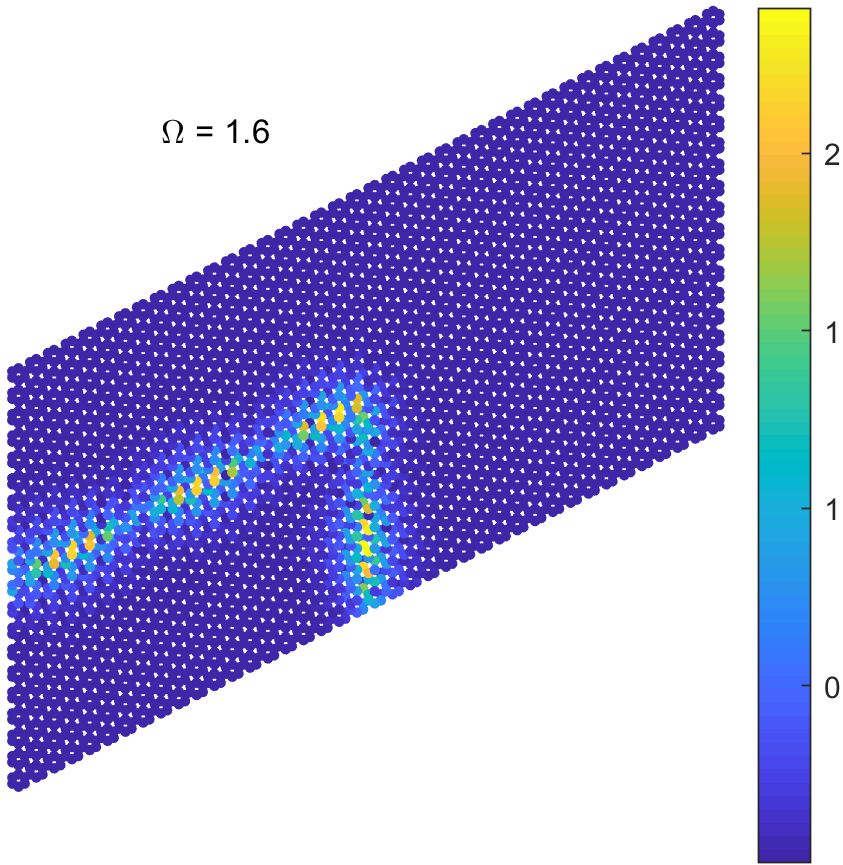
\includegraphics[width=1\linewidth]{imgs/sharpbendscat.png}
  \caption{The plot of $|y_i|$ for each mass in each cell.}
  \label{fig:sub2}
\end{subfigure}

\medskip
\centering
\begin{subfigure}[b]{.5\textwidth}
  \centering
  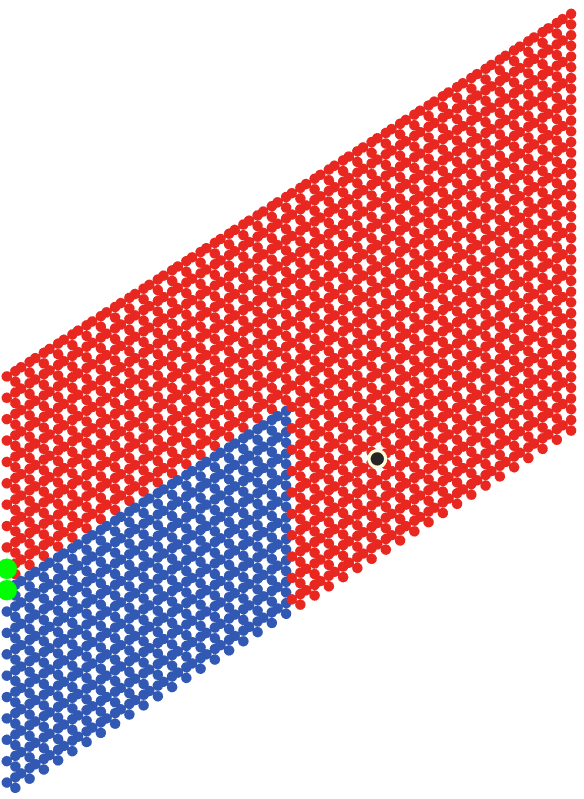
\includegraphics[width=0.8\linewidth]{imgs/kagomesharpbendarr.png}
  \caption{Arrangement of cells to form a sharp bend.}
  \label{fig:sub1}
\end{subfigure}%
\begin{subfigure}[b]{.5\textwidth}
  \centering
  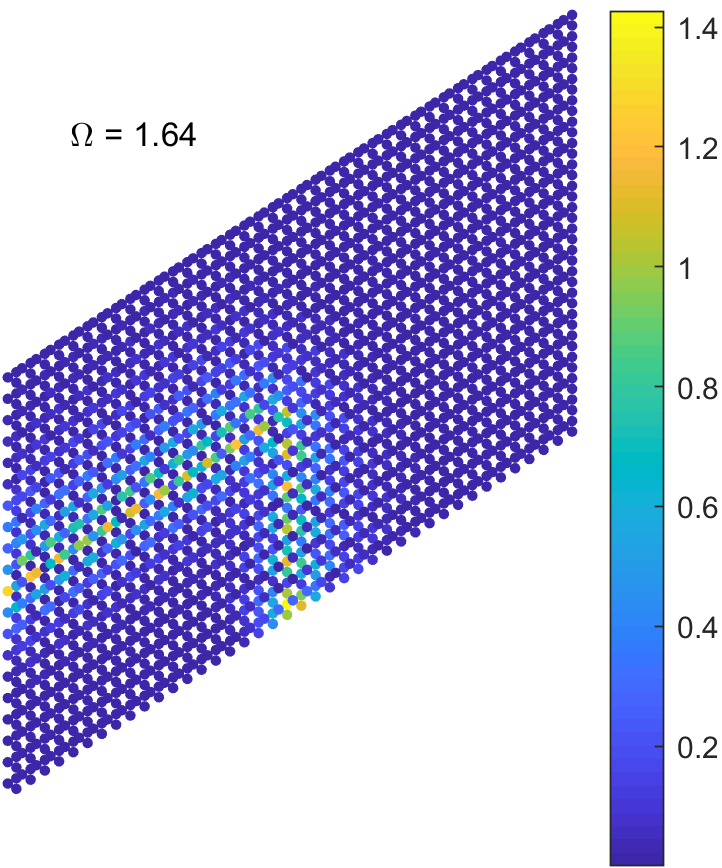
\includegraphics[width=1\linewidth]{imgs/kagomesharpbendscat.png}
  \caption{The plot of $|y_i|$ for each mass in each cell.}
  \label{fig:sub2}
\end{subfigure}
\caption{Simulation of scattering on the hexagonal and kagome finite lattice
  with a sharp bend.}
\label{fig:sharpbend}
\end{figure}

Amazingly, our systems are able to stand up to both of these bends as we can see
in Figure~\ref{fig:gentlebend} and Figure~\ref{fig:sharpbend}, and these type
of bends may be useful in the production of lenses.\cite{negrefraclens}

\section{Curved bends}
So it can travel around gentle and sharp straight bends; it is only natural to
then wonder if it can propagate as well along a curved bend. Being able to bend
energy around a corner could be useful in the creation of an invisibility
cloak.\cite{emcloak}

\begin{figure}[!h]
\centering
\begin{subfigure}[b]{.5\textwidth}
  \centering
  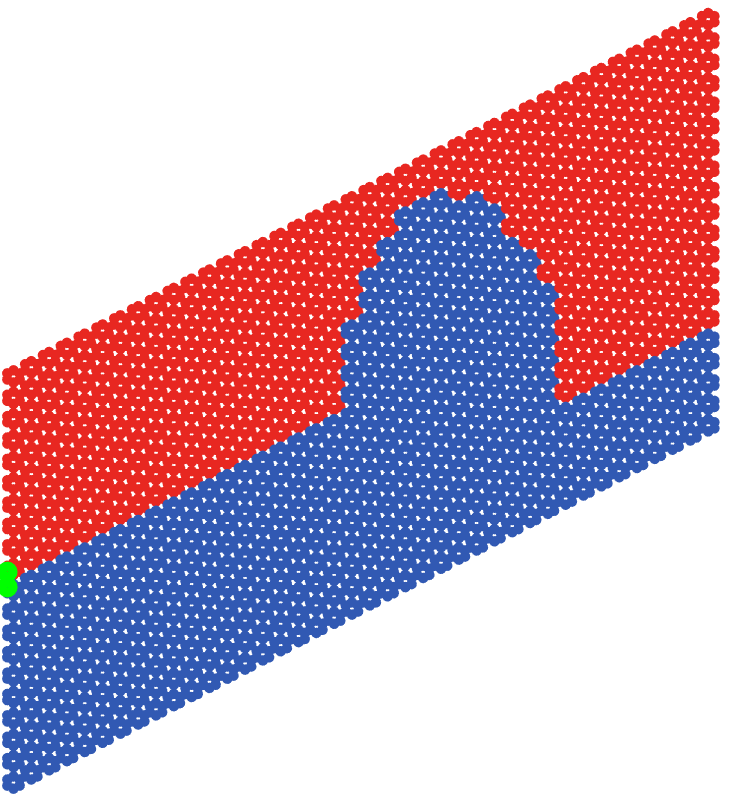
\includegraphics[width=0.8\linewidth]{imgs/curvedbendarr.png}
  \caption{Arrangement of cells to form a curved bend.}
  \label{fig:sub1}
\end{subfigure}%
\begin{subfigure}[b]{.5\textwidth}
  \centering
  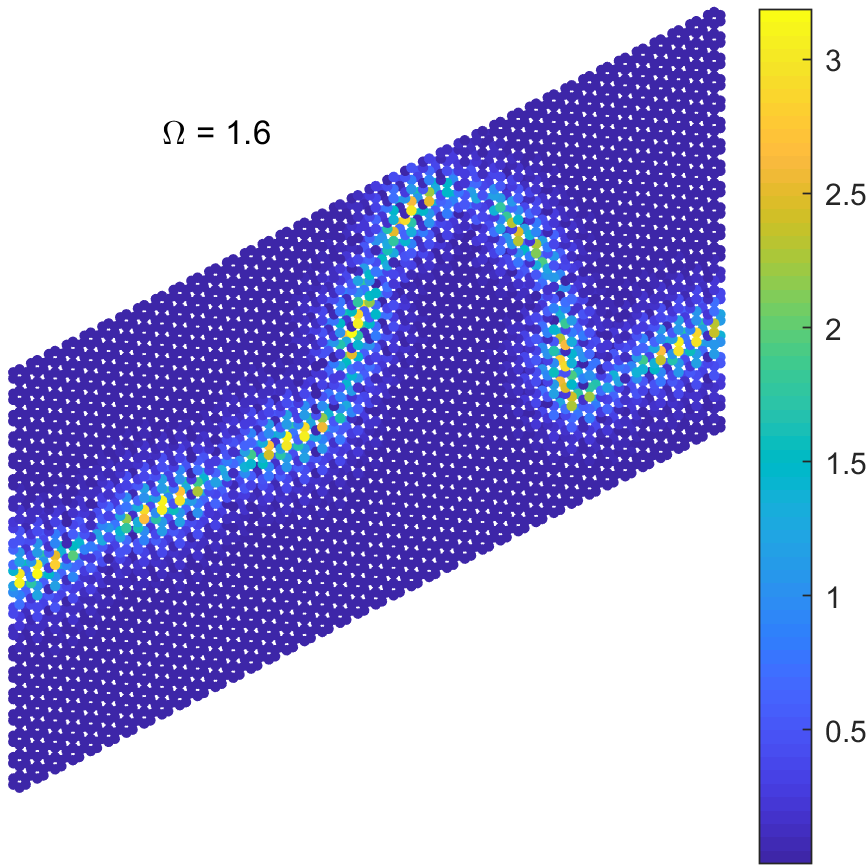
\includegraphics[width=1\linewidth]{imgs/curvedbendscat.png}
  \caption{The plot of $|y_i|$ for each mass in each cell.}
  \label{fig:sub2}
\end{subfigure}

\medskip
\centering
\begin{subfigure}[b]{.5\textwidth}
  \centering
  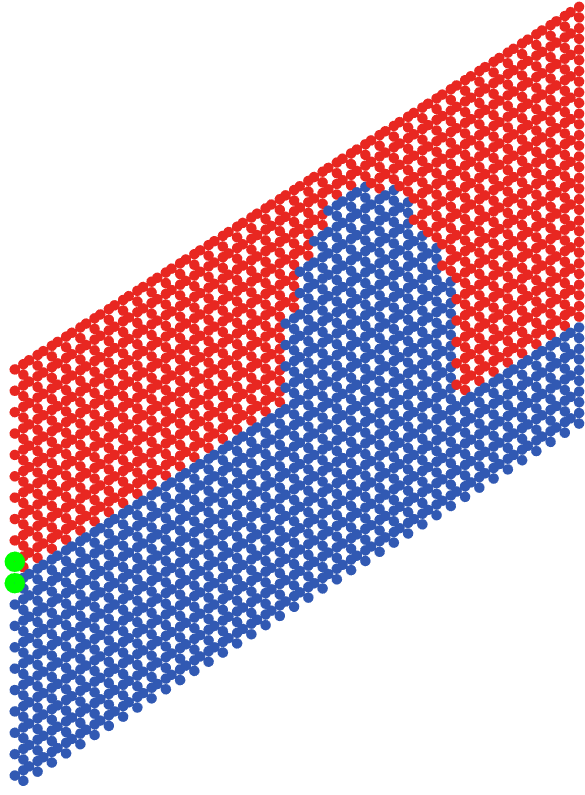
\includegraphics[width=0.8\linewidth]{imgs/kagomecurvedbendarr.png}
  \caption{Arrangement of cells to form a curved bend.}
  \label{fig:sub1}
\end{subfigure}%
\begin{subfigure}[b]{.5\textwidth}
  \centering
  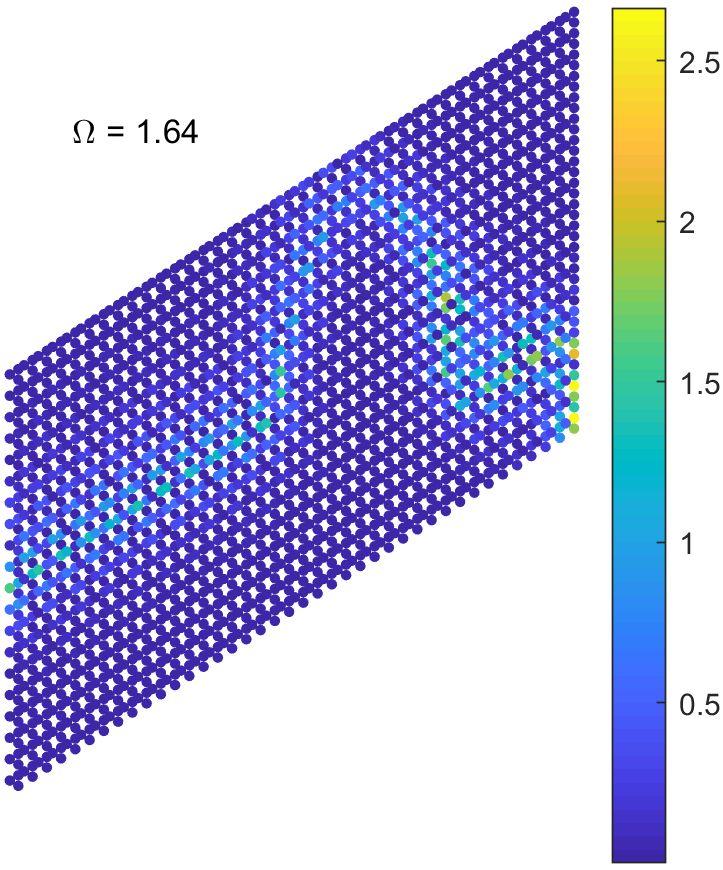
\includegraphics[width=1\linewidth]{imgs/kagomecurvedbendscat.png}
  \caption{The plot of $|y_i|$ for each mass in each cell.}
  \label{fig:sub2}
\end{subfigure}
\caption{Simulation of scattering on the hexagonal and kagome finite lattice
  with curved bend.}
\label{fig:curvedbend}
\end{figure}

\section{Energy splitting and merging}
One of the applications of metamaterials that we have discussed is splitting
and also focusing energy.\cite{toposplit,diremi,antennasol} And we see that we
are able to get the energy splitting behaviour in Figure~\ref{fig:esplit}.
Unfortunately we are unable to model the energy merging scenario in our system
as we do not model the flow of energy over time, but just the overall steady
state wave. However, we can imagine that we could have sources of excitation at
the three branches and have them converge onto the single branch.

\begin{figure}[!h]
\centering
\begin{subfigure}[b]{.5\textwidth}
  \centering
  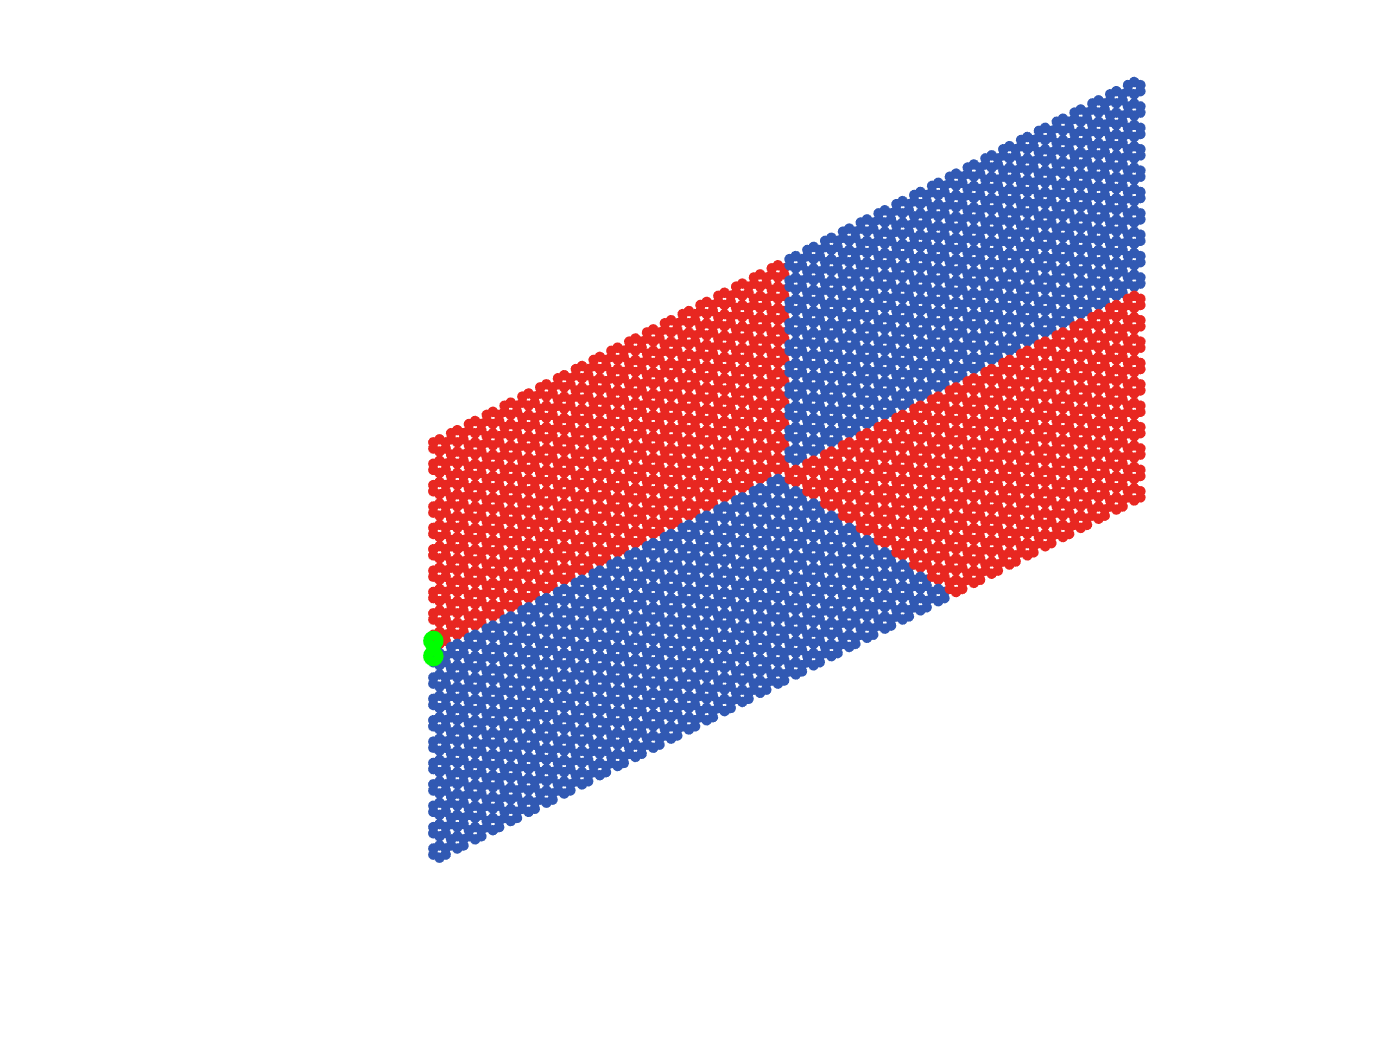
\includegraphics[width=0.8\linewidth]{imgs/esplitarr.png}
  \caption{Arrangement of cells to form a 3-way split.}
  \label{fig:sub1}
\end{subfigure}%
\begin{subfigure}[b]{.5\textwidth}
  \centering
  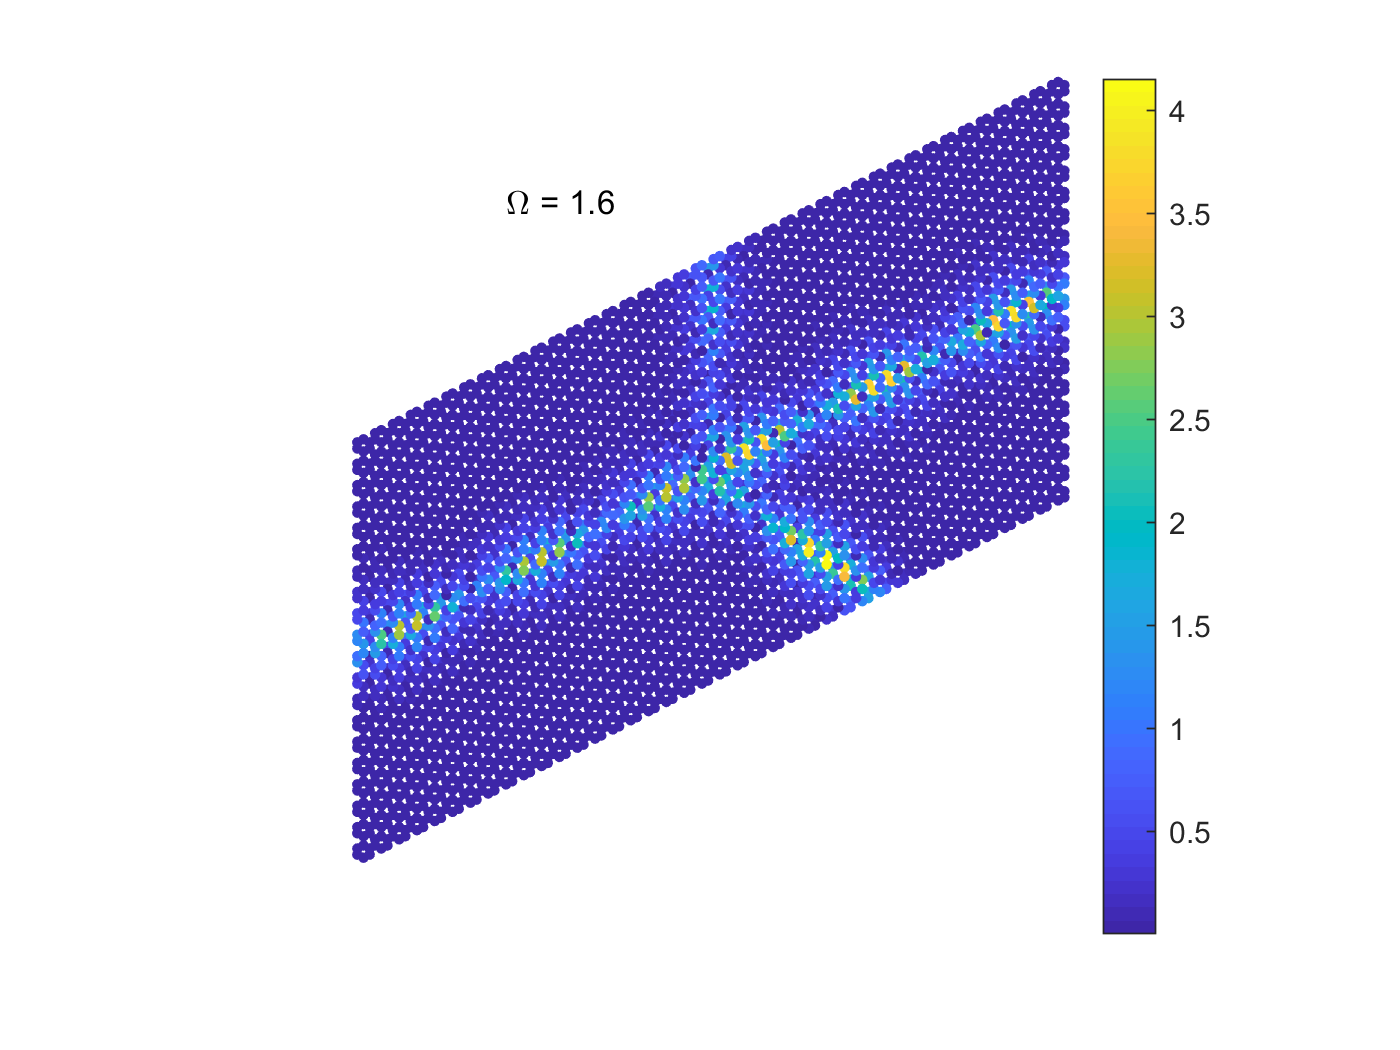
\includegraphics[width=1\linewidth]{imgs/esplitscat.png}
  \caption{The plot of $|y_i|$ for each mass in each cell.}
  \label{fig:sub2}
\end{subfigure}

\medskip
\centering
\begin{subfigure}[b]{.5\textwidth}
  \centering
  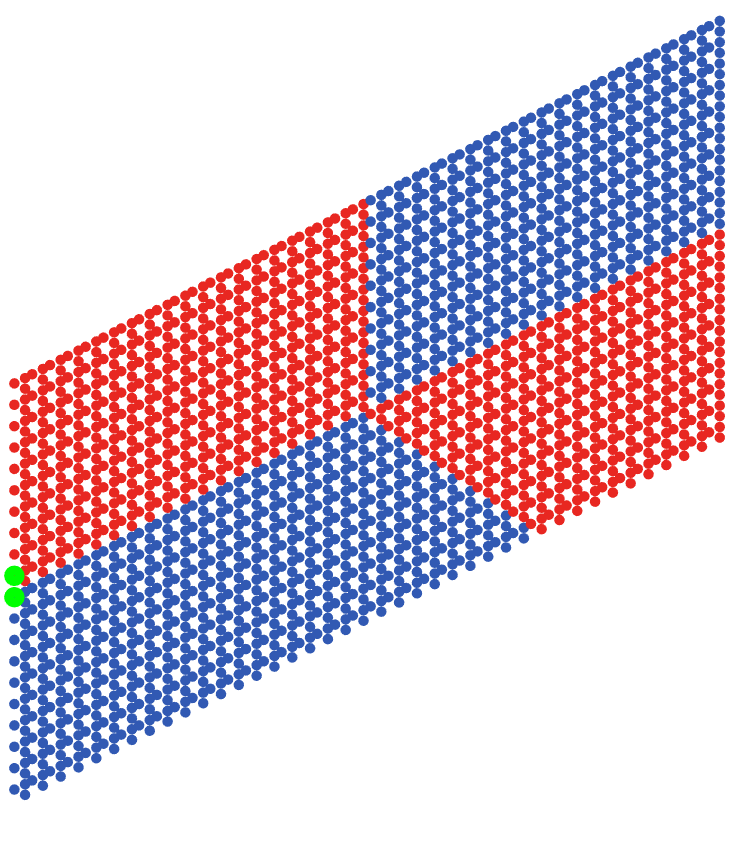
\includegraphics[width=0.8\linewidth]{imgs/kagomeesplitarr.png}
  \caption{Arrangement of cells to form a 3-way split.}
  \label{fig:sub1}
\end{subfigure}%
\begin{subfigure}[b]{.5\textwidth}
  \centering
  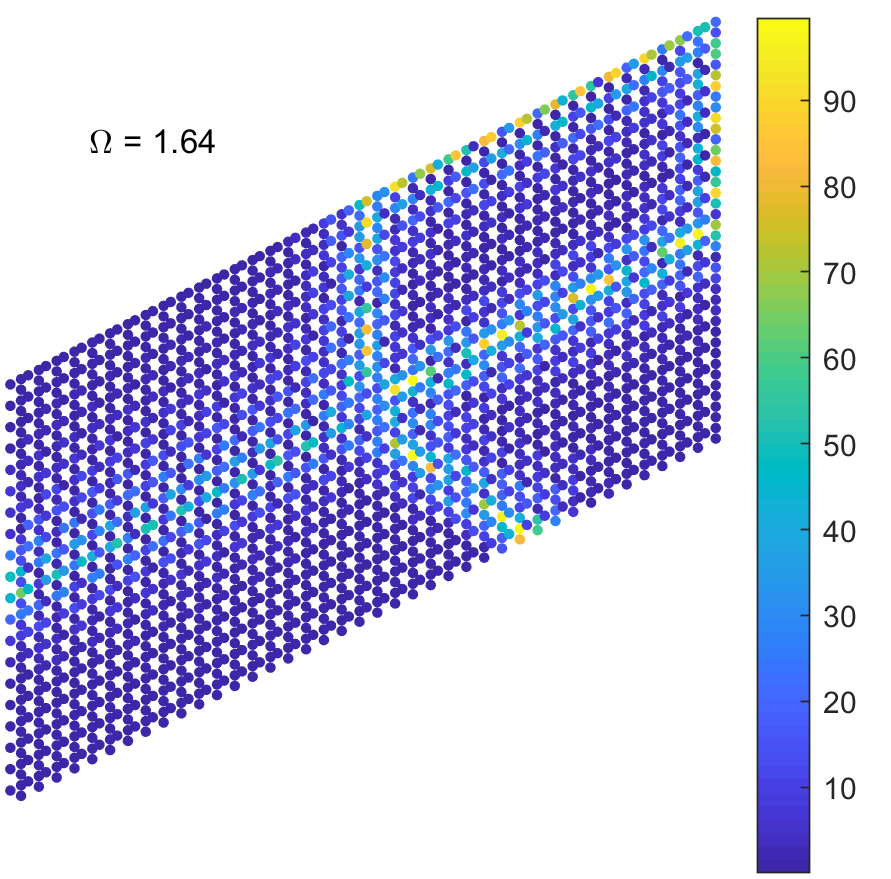
\includegraphics[width=1\linewidth]{imgs/kagomeesplitscat.png}
  \caption{The plot of $|y_i|$ for each mass in each cell.}
  \label{fig:kagomeesplit}
\end{subfigure}
\caption{Simulation of scattering on the hexagonal and kagome finite lattice
  with a 3-way split, modelling a 3-way energy splitter.}
\label{fig:esplit}
\end{figure}

